\chapter{Measuring distant objects with parallax}

%todo make two more telescopes on tripods, to have two setups going at a time. each group can use one telescope at a time, as long as scopes don't move.

%todo difference between measurement uncertainty and comparing between known and unknown quantities.


\section{Introduction}

Since it takes time for light to travel to us from objects in the universe, the further out an object is, the further back in time we see it. So for us to have an accurate picture of how the universe was in the past, we need to know how far away things are. For things that are nearby on Earth, we can travel there and see how far we went, or how long we took to get there. For things further away like the moon, we can use Kepler's laws, or we can bounce a beam of light off of it and see how long it takes to get back. For objects outside of our solar system, it would take too long, and the light would disperse too much, for us to use this last technique. For those objects that are still relatively nearby, we can use the parallax technique as the first rung on our distance ladder.

\section{Forming Groups}

If you are attending the lab session live and do not yet have a group, one way the TA could assist is to arrange "speed networking" among those who still need a group. This would involve the TA organizing Zoom Breakout Rooms, where each room is 2-3 students, and each group talks about how they work and what they are looking for in a group member. Then after 5 minutes or so, the Rooms are changed so people are with different people. This could help people get to know each other enough to form lab groups.

\begin{steps}
	\item Once you have a group, meet with each other and decide a) what tools you will use to communicate and collaborate, b) when you will meet, c) what you will do when you need to change an agreement, and d) what you will do when you a person has an issue with how the group is functioning.
%\textbf{Write this in your lab report. This part counts as data collection and analysis, so it can be identical in each member's report.}
\end{steps}

\section{Team roles}

\textbf{Decide on roles} for each group member. The available roles are:

\begin{itemize}
	\item Facilitator: ensures time and group focus are efficiently used
	\item Scribe: ensures work is recorded
	\item Technician: oversees apparatus assembly, usage
	\item Skeptic: ensures group is questioning itself
\end{itemize}

These roles can rotate each lab, and you will report at the end of the lab report on how it went for each role. If you have fewer than 4 people in your group, then some members will be holding more than one role. For example, you could have the skeptic double with another role. Consider taking on a role you are less comfortable with, to gain experience and more comfort in that role.

Additionally, if you are finding the lab roles more restrictive than helpful, you can decide to co-hold some or all roles, or think of them more like functions that every team needs to carry out, and then reflecting on how the team executed each function.

\section{Installing SAOImage DS9}

SAOImage DS9, or DS9 for short, is an image viewer, analyzer, and processor written and used by astronomers for working with astronomical images.

\begin{steps}
	\item Download and install DS9 from \url{http://ds9.si.edu/site/Download.html}. SAOImage DS9, or DS9 for short, is an image viewer, analyzer, and processor written and used by astronomers for working with astronomical images.
	
	If you click the link to download, it might say "redirecting" while never actually redirecting. In this case, copy the link into the address bar directly.
	\begin{framed}	
		\textbf{For MacOS}, unless you know otherwise, choose from the top set of choices (to the right of
		the blue apple logo). To find your version, from the Apple menu in the corner of the screen,
		choose “About This Mac”.
		
		If it displays a warning and prevents you from installed from an unidentified developer, follow the instructions at the following link to create an exception:
		
		\url{https://support.apple.com/guide/mac-help/open-a-mac-app-from-an-unidentified-developer-mh40616/mac}
	\end{framed}
\end{steps}

\section{Worksheet}

Complete the worksheet ``The Parsec'' on the following pages. You can draw the diagrams needed and include a picture of your diagrams, or use a drawing program to draw on them.
%Each member of the group will turn in their own worksheet as part of their lab report, and you can work in groups to complete them.

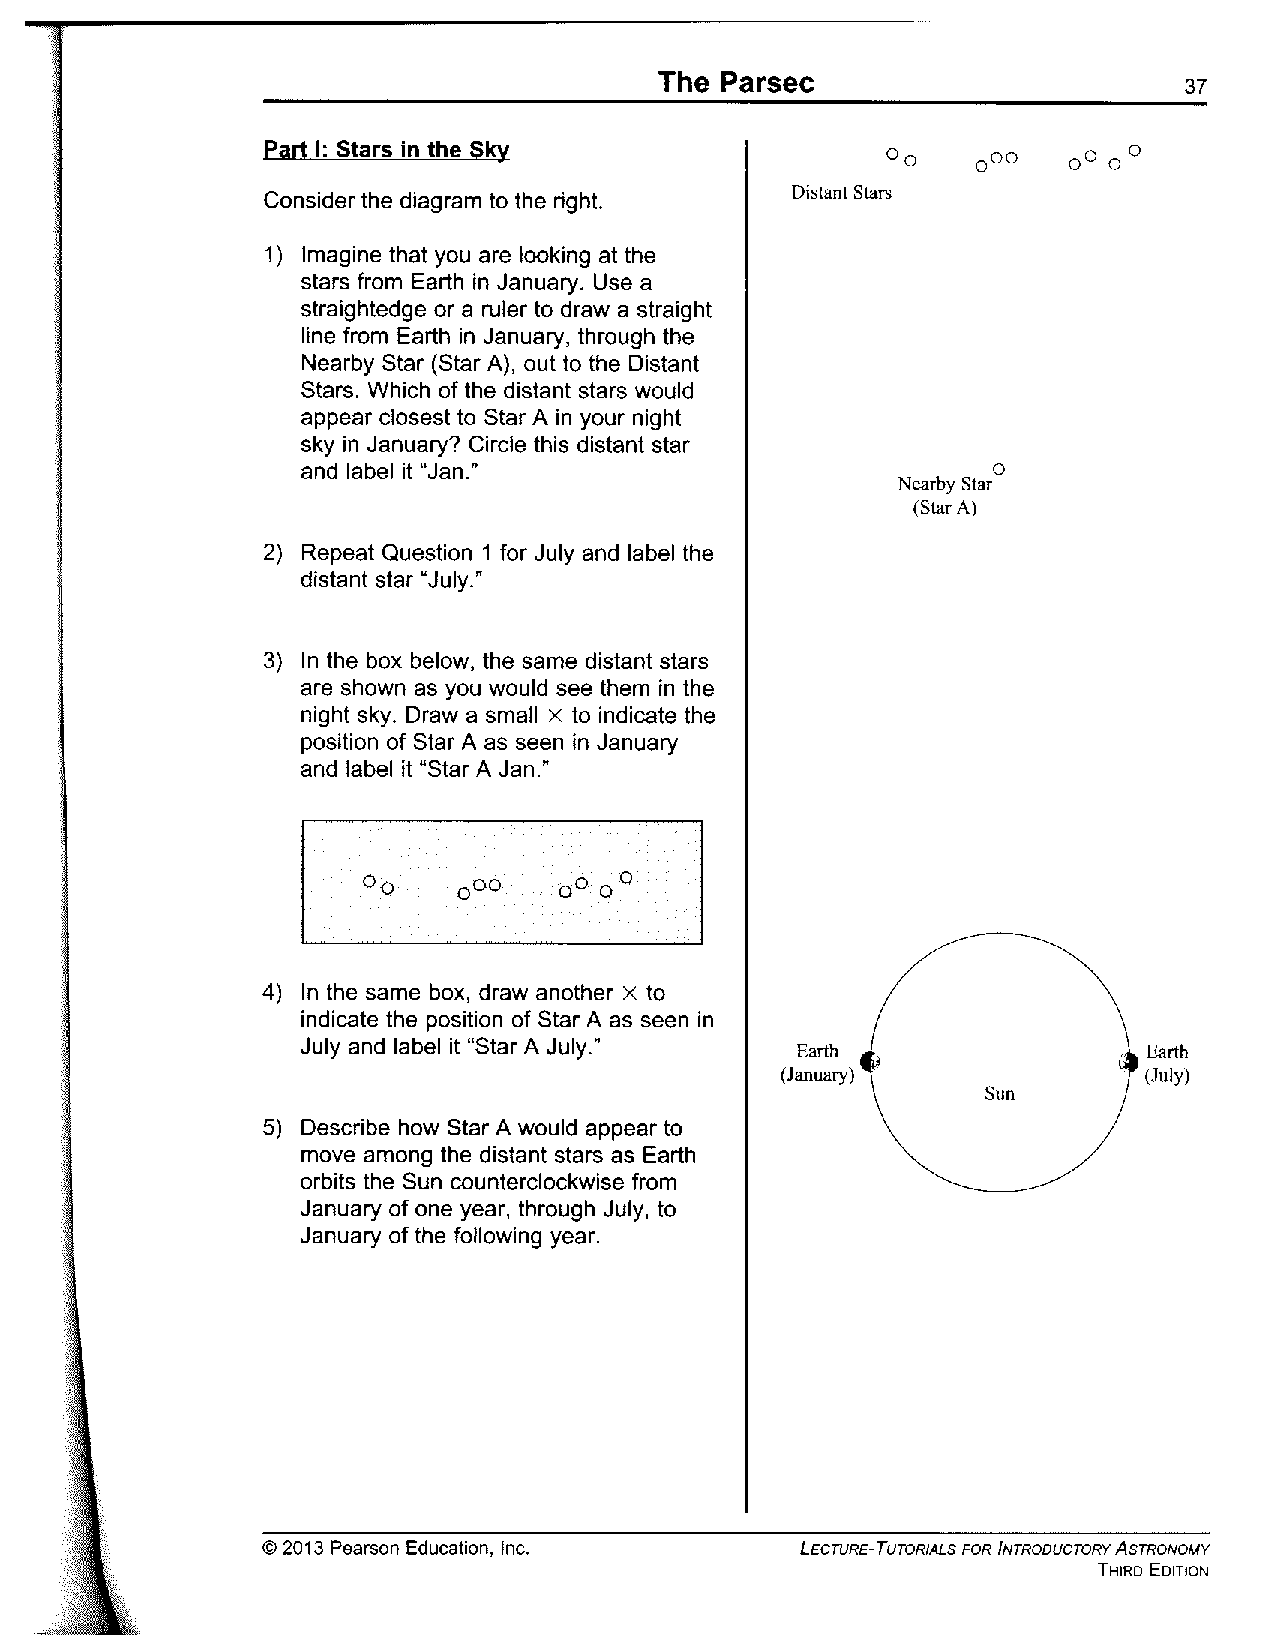
\includepdf[pages=1-2]{parallax/out.pdf}

\section{A quick measurement with hand tools}

You will now use the parallax technique to measure the distance to an object in your environment without needed to travel to it.

\begin{steps}
	\item Identify an object to be your ``nearby star'' and another as your ``distant star'', by analogy to the figure in the worksheet. Also choose the positions to view from as ``Earth (January)'' and ``Earth (July)''. When picking the stars and your Earth positions, check to see that from each Earth position, the distant star does not appear to move much, compared to the nearby star, and your guessed distance to the nearby star is at least 10 times greater than the distance between your two Earth positions.
\end{steps}
	
You'll first use crude measuring tools to compute the nearby star's distance with the parallax technique, and then use a more precise method. First, you'll use the little finger on your outstretched arm as a measurement of angular size --- the width of the index finger covers (``subtends'') about 1 degree.

\begin{steps}
	\item Identify an object to be your ``nearby star'' and another as your ``distant star'', by analogy to the figure in the worksheet. Find a place where you can stand and move a meter or two side to side and still see both ``stars''. The movement will simulate the Earth moving from its January to its July position. When picking the stars and your Earth positions, check to see that from each Earth position, the distant star does not appear to move much, compared to the nearby star, and your guessed distance to the nearby star is at least 10 times greater than the distance between your two Earth positions.
	
	\item Looking from just one eye, move so that the two stars appear to be directly overlapping. Mark your current position as Earth (January). Hold up your smallest finger at arm's length and move to your left or right until your finger fits just in between the two stars. This means that they are 1 degree away from each other in angular separation. Mark this position as Earth (July).
	
	\item Draw a diagram, similar to the second figure in the worksheet, and find your own Earth-Sun distance (half the distance between your Earth positions). Calculate the parallax angle in radians, which is half the 1 degree you measured with your finger. For the distance measurement, you can use a ruler, measuring tape, or objects that have standard lengths like coins, paper money, or sheets of paper (or Google Maps if the distance is very long, like for mountains or tall buildings in the distance).
\end{steps}
	
Now the distance to the nearby star can be found using the triangle formed by the line segments Sun-Earth, Earth-Star, and Star-Sun (see Figure~\ref{par:fig:figure}). Trigonometry relates these lengths to each other according to
\begin{equation}
	\tan p = \frac{a}{d}\,,
\end{equation}
where $p$ is the parallax angle in radians, $d$ is the distance to the star, and $a$ is half of the distance between the two measurement positions. Since the length $d$ is much greater than $a$, the angle $p$ is very small, and so we can use the small angle approximation $\tan u \approx u$, and therefore
\begin{equation}\label{par:eq:pad}
	p = \frac{a}{d}\,.
\end{equation}

\begin{figure}
	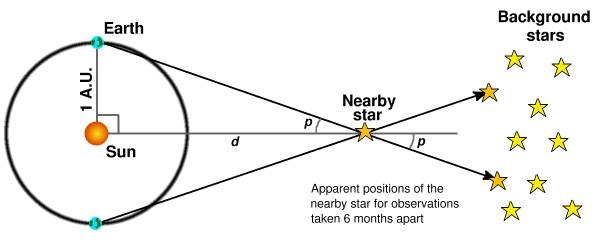
\includegraphics[width=\textwidth]{parallax/parallax-figure}
	\caption{Illustration of the geometry involved in a parallax measurement to determine $d$, the distance to a nearby star.}\label{par:fig:figure}
\end{figure}

\begin{steps}
	\item Use Equation\ \ref{par:eq:pad} to calculate the distance to the nearby star.
	
	\item Conduct the data collection twice more to get two more Earth-Star distances. You can use this to calculate the \textit{measurement uncertainty} --- the uncertainty is half the range of values, and the distance is the average of the 3 distances you found.
	
	\item Find the distance to the nearby star in a more direct way --- measure the distance with a measuring tape or pieces of paper, or for more distant objects, find them on Google Maps.
	For this value, also measure this distance 3 times and find the value and uncertainty as in the previous step.
\end{steps}

\begin{framed}
	\textbf{Notation for uncertain values}
	
To be precise about how imprecise our measurements are, scientists often express the quantities as ``$\langle \textrm{value} \rangle \pm \langle \textrm{uncertainty} \rangle$'', followed by the units. For example, if you measured your average distance to be 3.3 meters, and your uncertainty of that distance to be 0.4 meters, then to express in a succinct way, you can write the distance as ``$3.3 \pm 0.4\:$meters''.
\end{framed}

One way of describing how different two values are, without considering the uncertainty of those values, is to calculate the percent difference:
\begin{equation}
\textrm{percent difference} = \frac{d_1 - d_2}{\left(\frac{d_1+d_2}{2}\right)} \times 100\%
\end{equation}

\begin{steps}	
	\item How close is your parallax distance measurement to the direct measurement? Report the percent difference.
\end{steps}

In the next section, you will compare these values with each other using their uncertainties as well.

%Go out into the third floor hallway of KPTC (the long corridor near room 311).
%Go to the fifth floor of Eckhardt Research Center. Near the elevators on the north side, there are
%two telescopes%
% at the near end of the hallway, and an observing target is located at the far end.
%The target is a mock-up of the night sky, but with colors and relative sizes of objects greatly exaggerated to facilitate observations.

\section{Measuring with more precise equipment}

Using a finger for measuring angular separation is not very precise. Here you'll use the parallax technique to determine the same distance to the nearby star, but using a camera and analysis software instead.

%You will now use the telescope apparatus to measure the parallax of a “foreground star”
%(actually a ball on a stick)
%(actually a nearby building), with the
%mock-up star field
%Chicago skyline
%serving as “background stars.”
%Place the “foreground star” part way down the hallway between the telescopes and the observing target.
\begin{steps}
	\item Take a picture from a digital camera (likely your phone camera) from the vantage point of each Earth position used above.
	
	
%Make sure that it is positioned so that sightlines from both telescopes
%pass through both the “foreground star” and the “background stars,”
%(an overlapping background of the skyline).
%With your smartphone, take an image of the “foreground” and “background” stars through each telescope.
%Also measure the distance between the two telescopes using a measuring tape and record
%this value in your lab notebook. See Figure~\ref{par:fig:images} for example data.

%\begin{figure}
%	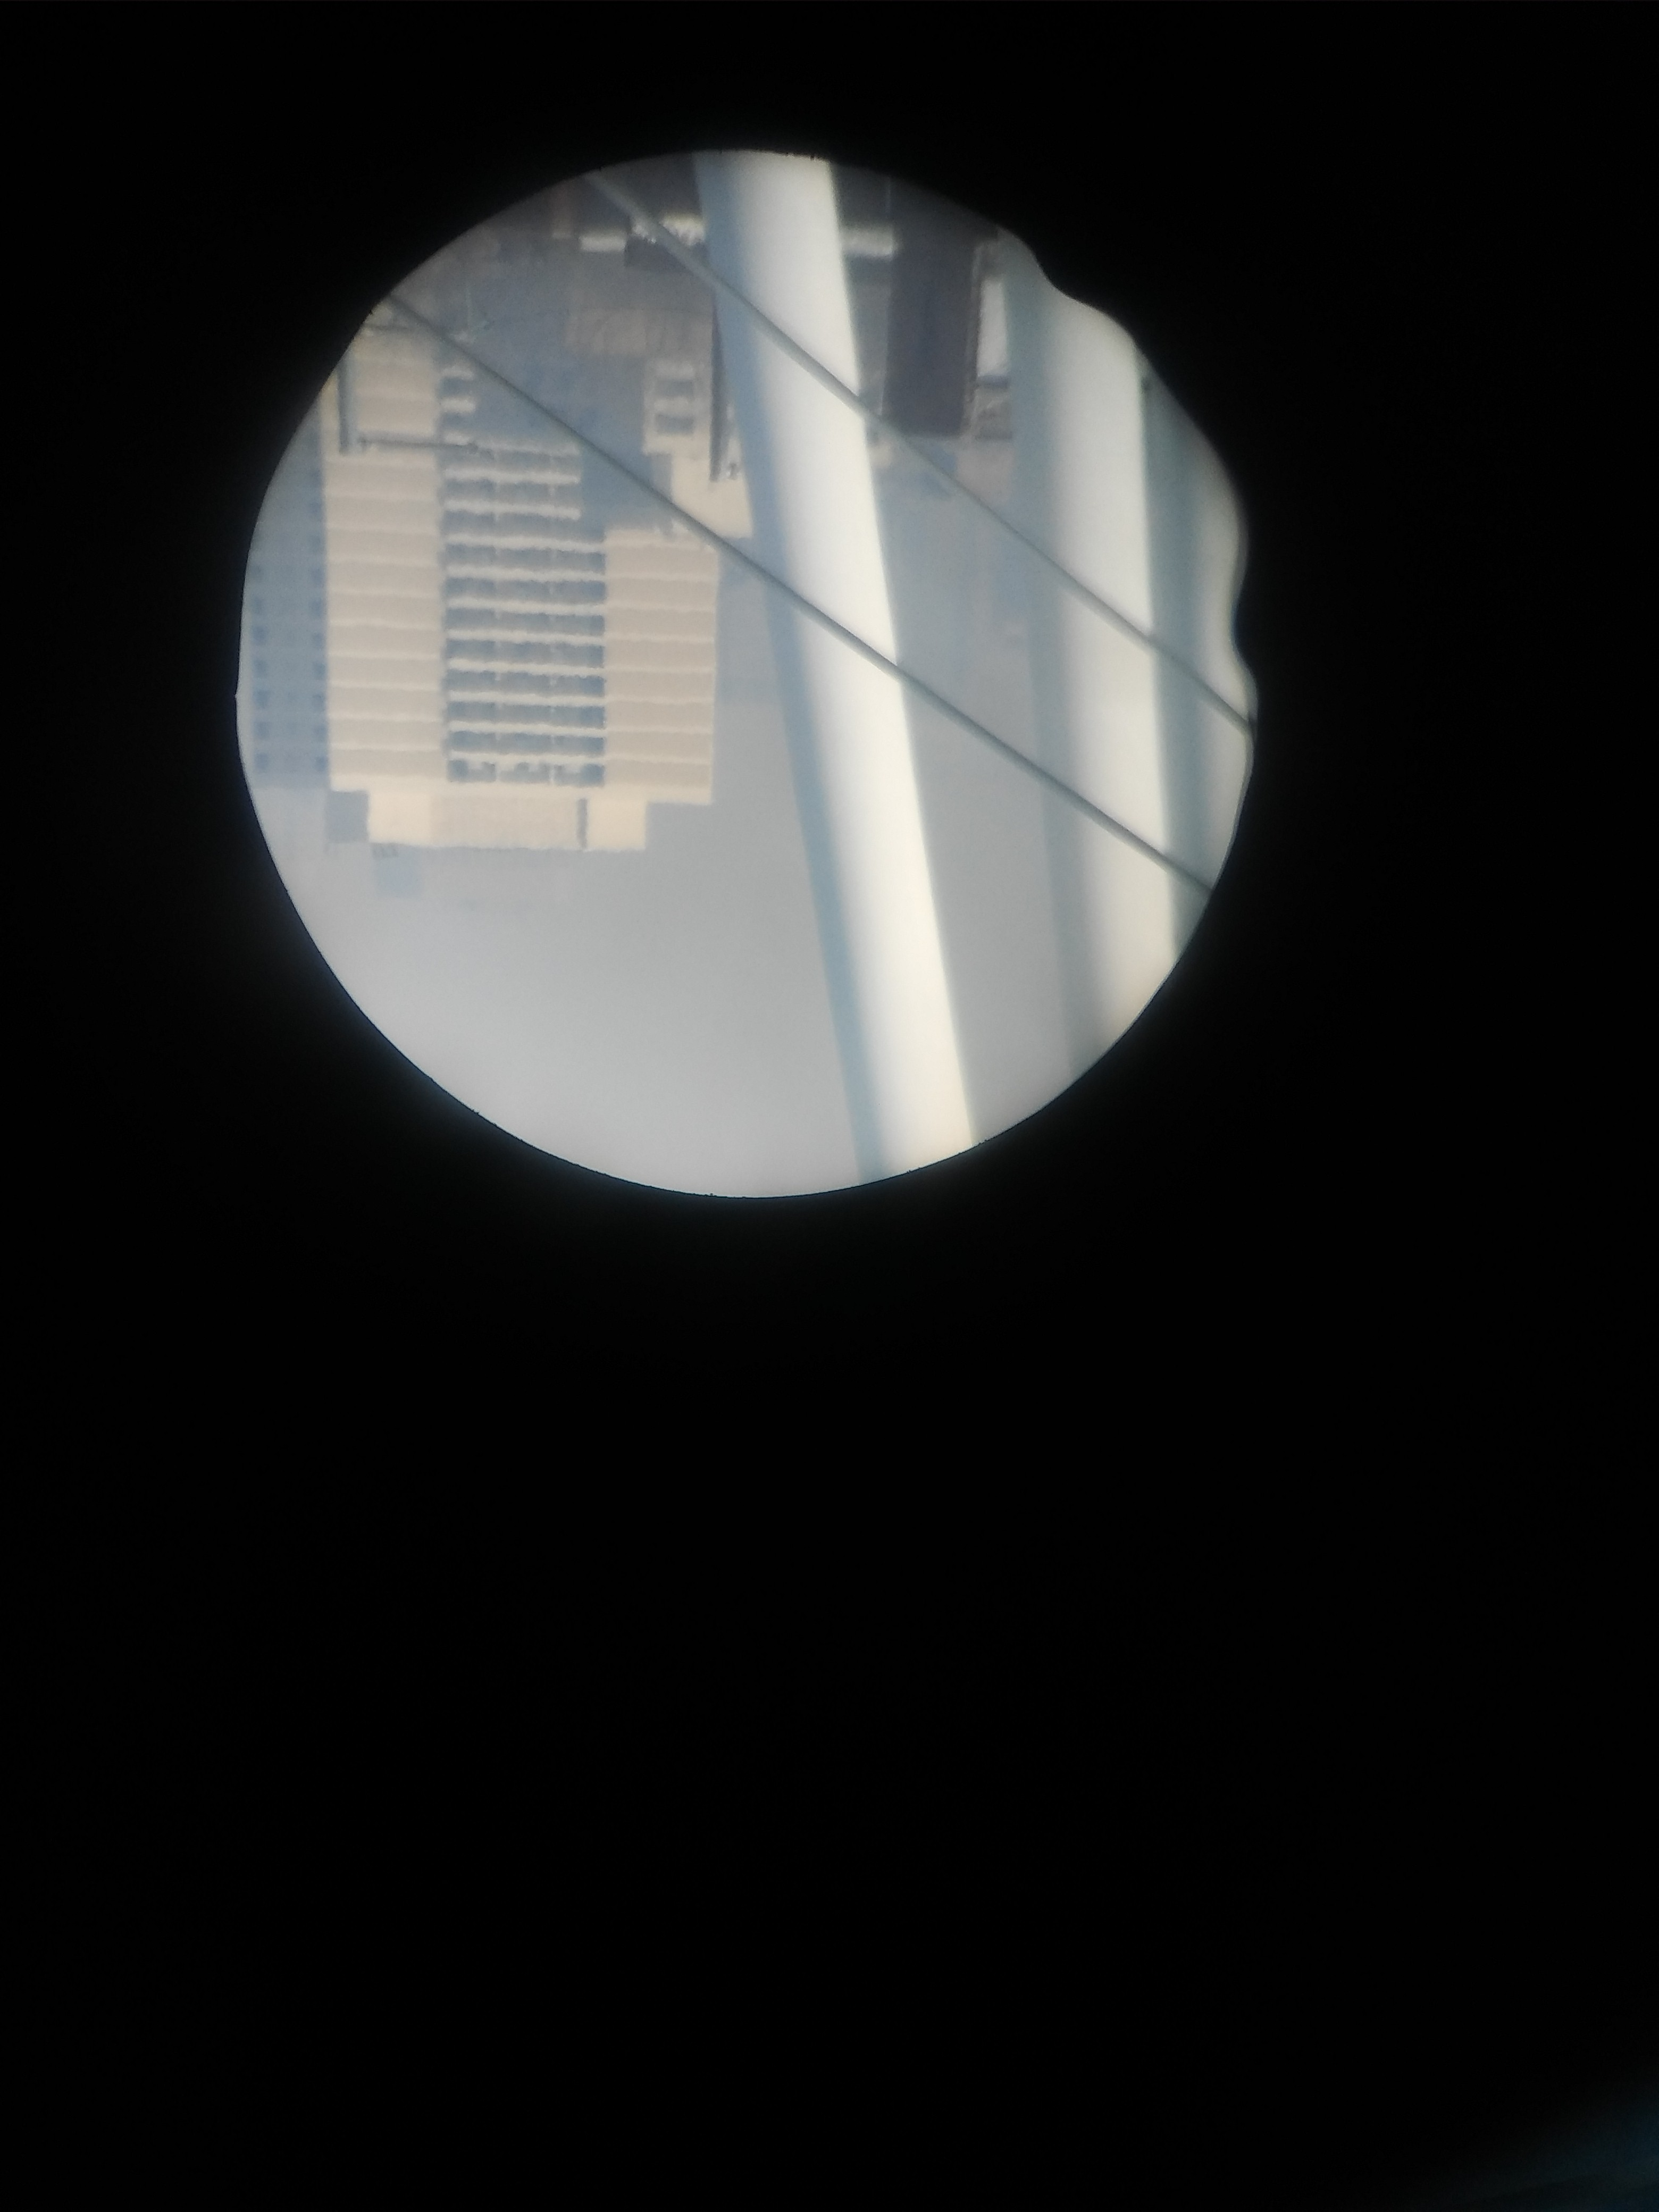
\includegraphics[width=0.5\textwidth]{parallax/parallax-image-1}
%	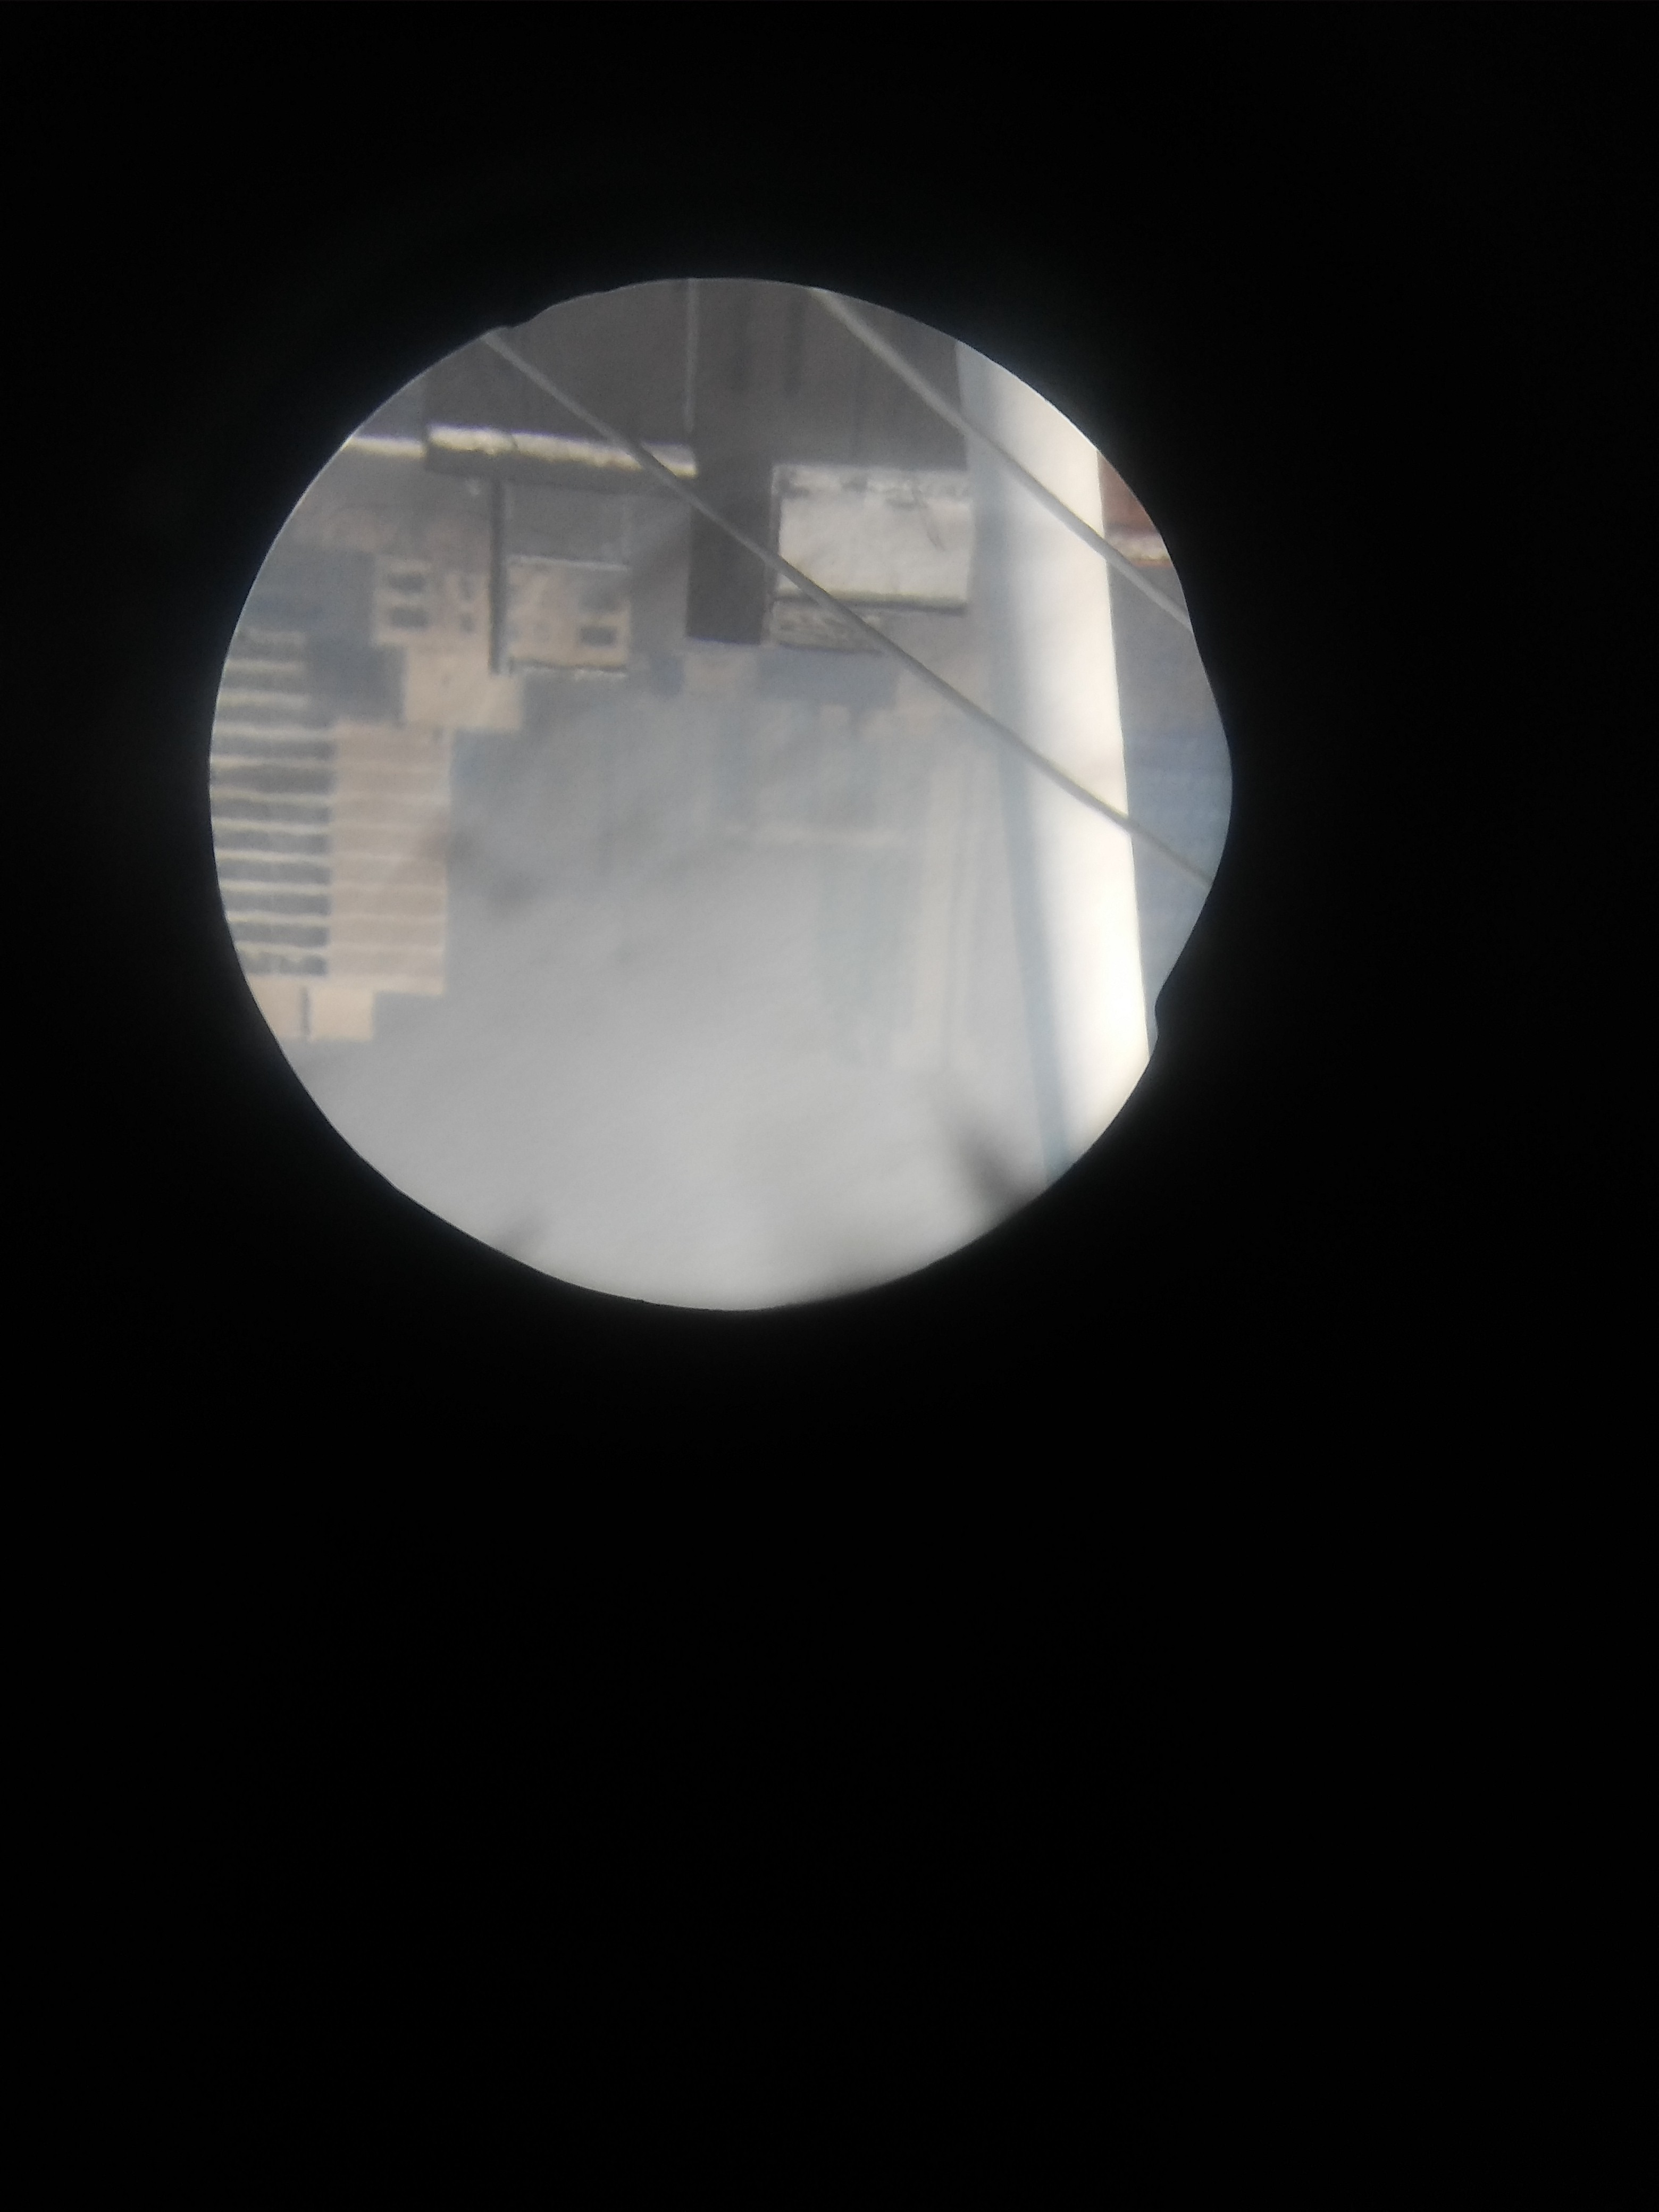
\includegraphics[width=0.5\textwidth]{parallax/parallax-image-2}
%	\caption{Example images. My foreground ``star'' was the point defined by the left intersection of the lower cable and the white pillar on top of the gym on campus. One of my reference ``stars'' was the top right corner of the building in the background. Note that the images produced by this telescope are upside down.}\label{par:fig:images}
%\end{figure}

%You have now finished collecting data, so now it’s time to analyze it. 
	\item Upload your photographs to a computer. The simplest way to do this may be to email the images to yourself from your phone. Give each file a descriptive name (e.g. ``\texttt{parallax\_left\_telescope}'').
\end{steps}

\subsection{Finding the pixel scale}

Notice that with the finger, I told you that your little finger, outstretched, is about 1 degree wide. This was a conversion between the linear size of your finger, for example 1 cm, to an angular size, 1 degree. With the camera, we need to find out the similar conversion --- how many pixels in an image corresponds to what angular size, also known as the \textit{pixel scale} of the image. To do this, you can take a known angular size and measure its length in pixels.
\begin{steps}
	\item Find an object of known length and place it a known distance from the camera (distance to camera should be 10 times or more the length of the object). Take a picture of that object.
\end{steps}

You will now convert the images from their default format (likely .png or .jpeg) into .fits
files, a format commonly used by astronomers. This format will be readable by SAO
Image DS9, an astronomical image analysis tool.
\begin{steps}
	\item Convert the image files to a .fits format using your favorite image processing software, or the software ``GIMP'' (Gnu Image Manipulation Program), or an image conversion website like \url{https://www.files-conversion.com/image/fits}. For using GIMP, open the file. From the FILE menu, select EXPORT AS, change the
file extension to “.fits,” and then click EXPORT. Repeat this procedure for each of your
images.

\item Open a saved .fits image of the pixel scale image in DS9. Your first task is to measure the pixel scale.
%Adjust the contrast so you can clearly see the field of view.
From the menu at the top of the screen, select REGION, SHAPE, LINE. On the first row
of buttons in the DS9 window, click EDIT then on the second row click REGION. Draw
a line along the known length of the object. On the first row of buttons, click REGION then on the
second row click INFORMATION. A window should pop up that will give you the length
of the line in physical units, that is, in pixels. \textbf{Record this value in your lab notebook.}

\item Find the angular size of the known object. Since the object is far away, we can again use the small angle approximation for the triangle involved and find that the angular size of the object is equal to its length divided by the distance to the object. This angle is in radians.

\item Find the pixel scale by dividing the number of pixels in the length by the angular size of the known object. This gives the pixel scale in pixels per radian.

\end{steps}
\subsection{Finding the parallax angle}

Now that you have the pixel scale of the image, you can use that to measure the parallax angle of the your nearby star and thus find the distance to that object like you did with the little finger method.

\begin{steps}
	\item Open the first parallax image. Measure the displacement from the nearby star to the distant star. Convert that displacement to radians using the pixel scale. Make sure to record both the X- and Y- offsets. Repeat these measurements for the second parallax image using the same distant star.

	\item Find the total angular distance the star moved between images. To do this, subtract the X- offsets from each other, and subtract the Y- offsets from each other. Then use the Pythagorean theorem to find the total distance moved ($d = \sqrt{x^2 + y^2}$). Divide this by two to get the parallax angle.
	
	\item Use Equation\ \ref{par:eq:pad} to find your new calculation for the distance to the nearby star.
	
	\item Calculate the percent difference between this and the direct measurement like you did in the previous section.
	
	\item Use the $t'$ statistic described in Appendix\ \ref{unc:sec:comparing} to compare the two values and interpret the result --- do these two ways of distance measurement really measure the same thing?
\end{steps}

%Given that the field of view of the Galileoscope is 1.5\textdegree
% (0.75\textdegree with the Barlow eyepiece)
%calculate the \textit{plate scale} of your images, in arcsec/pixel.

%Select a reference star from your parallax measurements. Using your plate scale,
%determine the angular separation between the reference star and the target star. Record
%the value for the total separation, $r$, and for both the horizontal ($x$) and vertical ($y$) components. You can
%check your measurements against each other by inputting these values into the
%Pythagorean formula: $r^2 = x^2 + y^2$. Do your measurements agree?
%
%Repeat the above calculations for all reference stars in both of your parallax images. You
%can now calculate the distance to the foreground star. The distance to a star can be found using the triangle formed by the line segments Sun-Earth, Earth-Star, and Star-Sun (see Figure~\ref{par:fig:figure}). Trigonometry relates these lengths to each other according to
%\begin{equation}
% \tan p = \frac{a}{d},
%\end{equation}
%where $p$ is the parallax angle in radians, $d$ is the distance to the star, and $a$ is half of the distance between the two measurement positions. Since the length $d$ is much greater than $a$, the angle $p$ is very small, and so we can use the small angle approximation $\tan u \approx u$, and therefore
%\begin{equation}
%p = \frac{a}{d},
%\end{equation}



%Use each reference star to calculate an independent measurement of parallax. To do this, for each reference star, you'll need to find how far (in radians) the target star has moved between the two observations. Using vector arithmetic\footnote{See \url{https://www.mathsisfun.com/algebra/vectors.html} for a short tutorial}, subtract the two displacement vectors from each other by components and find the magnitude of that difference vector. Divide by 2 and convert to radians to find $p$. After finding $p$ from each reference star, average these values together and estimate your uncertainty by finding the standard deviation of these measurements. You can perform this calculations in Excel using the functions AVERAGE() and STDEV(). Report your measurements in a table in your lab
%report.
%
%Also use a map to find the distance from you to your foreground star (with uncertainty). Compare these quantities with their uncertainties using the procedure found in Appendix~\ref{unc:sec:comparing}, to see the degree to which they agree.

%\section{Questions}\label{par:sec:questions}
%
%These should be included in your lab report.
%
%\begin{steps}
%	\item Your parallax measurements depend on an incorrect implicit assumption. What is
%	this assumption, and how will it bias your results? How would you change the
%	procedure in order to minimize this bias?
%	\item What were the primary sources
%	of uncertainty? How would you improve the procedure for future measurements?
%\end{steps}

\section{Report checklist}

Include the following in your lab report. See Appendix~\ref{cha:lab-report-format} for formatting details. Each item below is worth 10 points.

\begin{enumerate}
	\item Your group's agreements about communication.
	\item The completed worksheet ``The Parsec''.
	\item Work and final answer for your distance measurements using your finger, with uncertainty.
	\item Work and final answer for direct distance measurement, along with percent difference.
	\item A figure with your three images (pixel scale image and two parallax images).
	\item The displacement vectors from distant star to nearby star.
	\item Final determined value of the distance and comparison with the direct distance using percent difference and $t'$ statistic. Show your work (see Appendix~\ref{cha:lab-report-format}).
%	\item Answers to the questions in Section~\ref{par:sec:questions}, with justification.
	\item A 100--200 word reflection on group dynamics and feedback on the lab manual. Address the following topics: who did what in the lab, how did you work together, how group roles functioned, what successes and challenges in group functioning did you have, and what would you keep and change about the lab write-up?
\end{enumerate}